%!TEX program = xelatex

\documentclass[12pt]{ctexbeamer}
\usepackage[ustcblue]{ustcbeamer}%可通过更改选项来更改主题颜色
\usepackage{listings}

%%%模板说明%%%%
%模板ustc_beamer中定义了五个选项供选择:ustcblue,ustcred,black,violet,blue;分别对应了五种主题颜色。
%建议使用ustcblue和ustcred,两者均为科大党委宣传部规定的校徽标准配色,参考http://lswhw.ustc.edu.cn/index.php/index/info/3370 。两个标准配色分别为:蓝cmyk(100,80,0,0)、红cmyk(0,100,100,0),在LaTex中使用需要除以100。
%本模板参考了https://github.com/thomasWeise/ustcSlides 的Slides,故而保留了Thomas Weise先生的原始配色(blue)。
%不怎么建议使用黑色(black),看上去像讣告。
%有其他的配色需求可在github上反馈。
%%%%%%%%%%%%%%%%%%%%%%%%%%%%%%%%%%%%%%%%%%%%%%%%%%%%%%%%%%%%%%%%%%%%%%

\title[神经网络计算库运行时优化]{
    面向神经网络计算库的运行时\\
    优化技术研究与实现
}
\author[徐文明]{报告人:徐文明}
\institute[USTC]{
中国科学技术大学,软件学院\\
实习单位:北京中科寒武纪科技有限公司
}
\date{\today}

\begin{document}

\startPresentation{}

\AtBeginSection[]{
  \begin{frame}%
    \frametitle{大纲}
    \tableofcontents[currentsection]
  \end{frame}
}

\section{问题分析}
\begin{frame}
  \frametitle{问题分析}
  \begin{block}{场景描述}
    \begin{itemize}
    \item 一家酒店想在前台的嵌入式设备上部署深度学习的人脸识别应用来登记和核对入住客户的身份信息,结果发现嵌入式设备上硬件资源有限,无法编译深度神经网络应用程序。
    \item 一个算法研究员为了调试某个神经网络的正确性,不断改变神经网络的权值数据,结果每改变一次,整个网络就需要重新编译运行。研究员不得不花费大量时间在网络的编译过程上。如果该研究员很细心,每次调整权值后都保存一份对应的神经网络模型,不久系统出现存储空间不足的提示,原因是神经网络模型体积太大。。。
    \end{itemize}
  \end{block}
\end{frame}

\begin{frame}
  \frametitle{问题分析}
  \begin{block}{用户故事分解}
    \begin{itemize}
    \item “想要在资源有限的设备上部署深度学习应用”
    \item “想要加速神经网络的编译运行过程”
    \item “想要减小神经网络模型的体积”
    \end{itemize}
  \end{block}
\end{frame}

\begin{frame}
  \frametitle{问题分析}
  \begin{block}{针对上述问题的思路}
  	 我们需要深度学习加速库具有以下的功能:
    \begin{itemize}
    \item 支持动态重新编译,能在Host端编译,在设备端部署,即“离线运行模型”模式
    \item 能够避免相同神经网络的重复编译
    \item 能够压缩神经网络的体积,减少存储和部署时的资源占用
    \end{itemize}
  \end{block}
\end{frame}

\section{背景技术}
\begin{frame}
  \frametitle{背景技术}
  \begin{block}{研究背景与方向}
  \begin{enumerate}
    \item 运行时优化
    \item DNNCL的编程模型
    \item 权值量化
  \end{enumerate}
  \end{block}
\end{frame}

\begin{frame}
  \frametitle{背景技术}
  \begin{block}{1.运行时优化}
     在程序运行的过程中采集和分析程序的运行时信息,对程序中执行频率较高的代码片断进行优化,从而加速程序运行。
    \begin{itemize}
    \item 优化热点区域
    \item 减小运行时开销
    \end{itemize}
  \end{block}
\end{frame}

\begin{frame}
  \frametitle{背景技术}
  \begin{block}{2.DNNCL的编程模型}
    \begin{itemize}
    \item 使用符号张量图描述网络模型,便于添加新的层,拓展性好
    \item 使用符号式编程,先声明一张计算图来声明整个计算过程,接着编译,最后执行具体计算任务,便于优化,效率高。
    \end{itemize}
  \end{block}
\end{frame}

\begin{frame}
  \frametitle{符号张量图}
  \begin{columns}
    \begin{column}{0.50\textwidth}
       \begin{figure}
		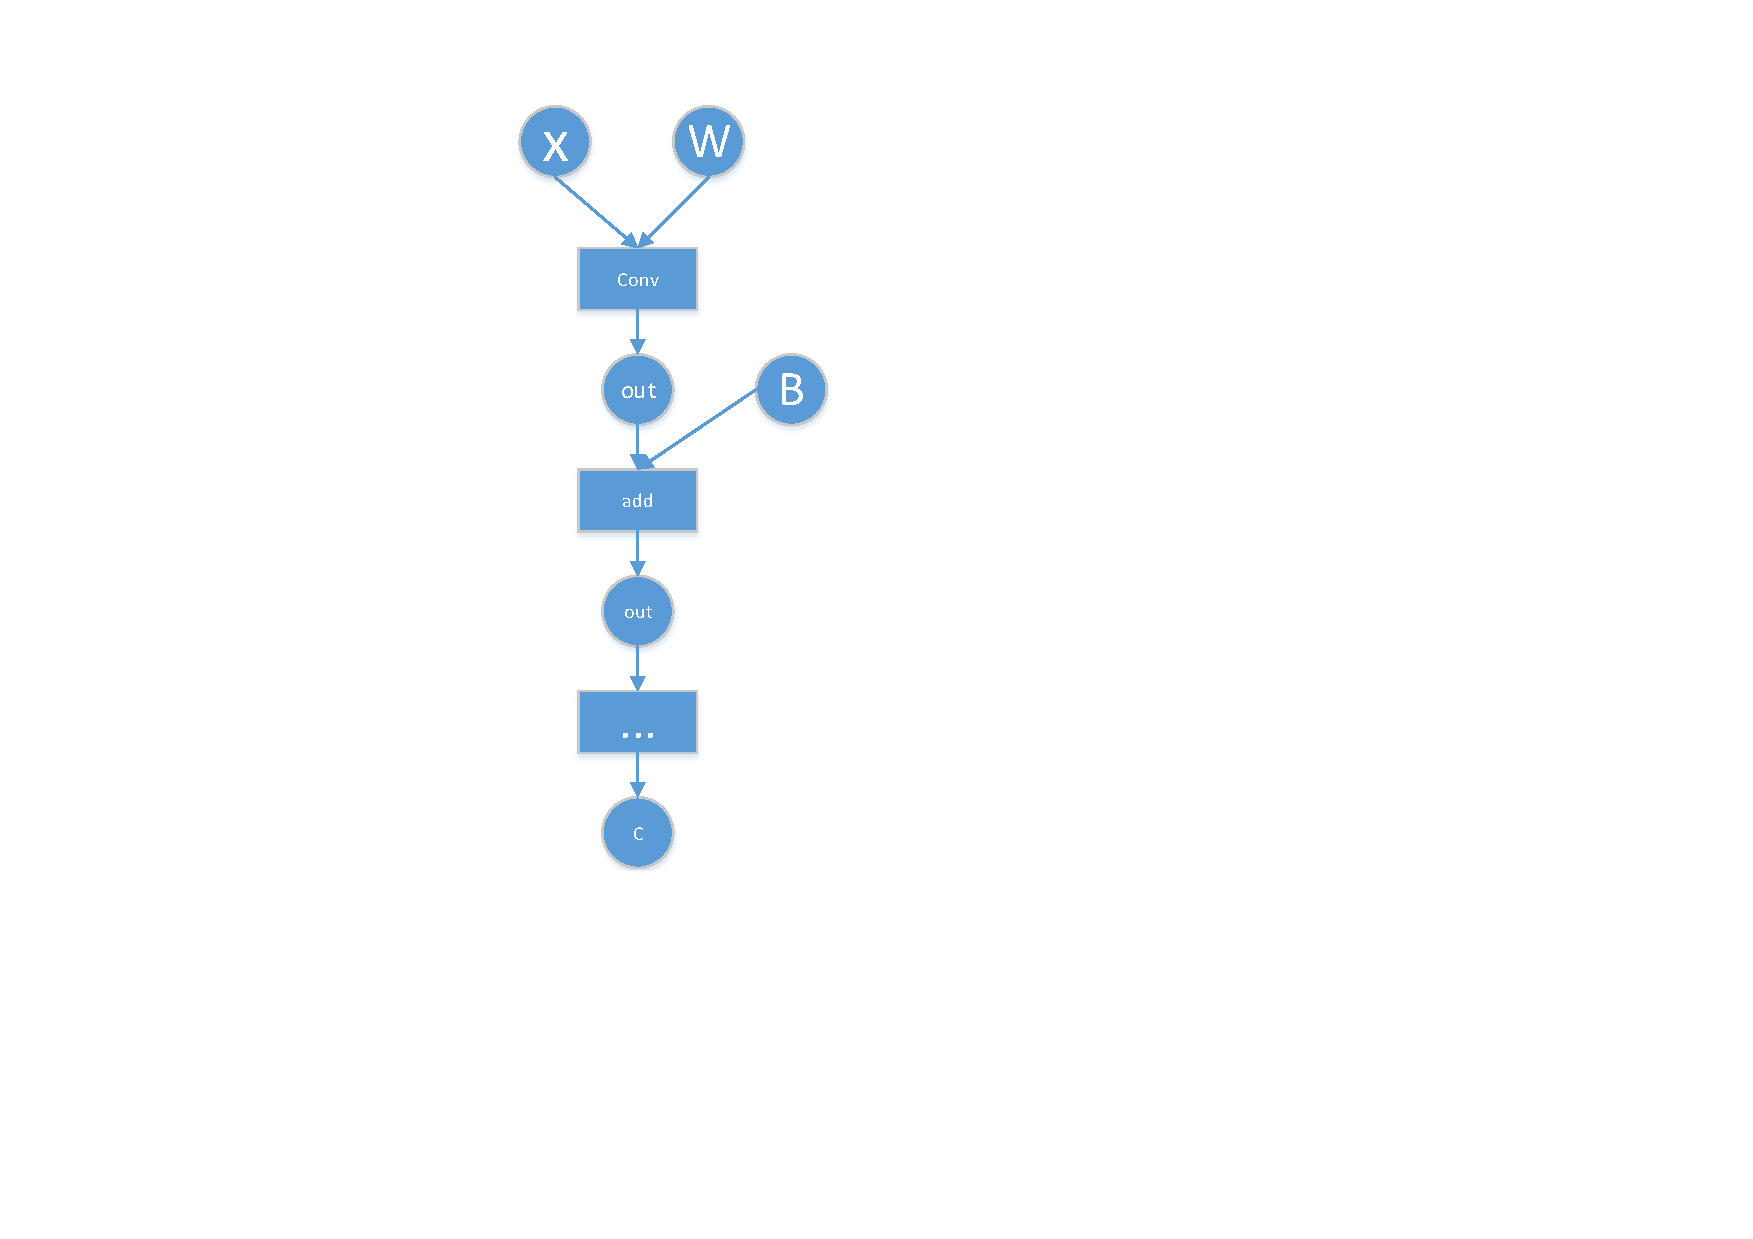
\includegraphics[width=0.3\textwidth]{figures/computing_graph.pdf}
       \end{figure}
    \end{column}    
    \begin{column}{0.50\textwidth}
    \begin{block}{核心数据结构}
       \begin{itemize}
          \item 张量(Tensor):input/output, bias, filter
          \item 操作(Operation):conv, add, mlp, concat, split...
        \end{itemize}
      \end{block}
    \end{column}
  \end{columns}
\end{frame}

\begin{frame}
  \frametitle{用户编程模型}
  \begin{columns}
    \begin{column}{0.50\textwidth}
       \begin{figure}
		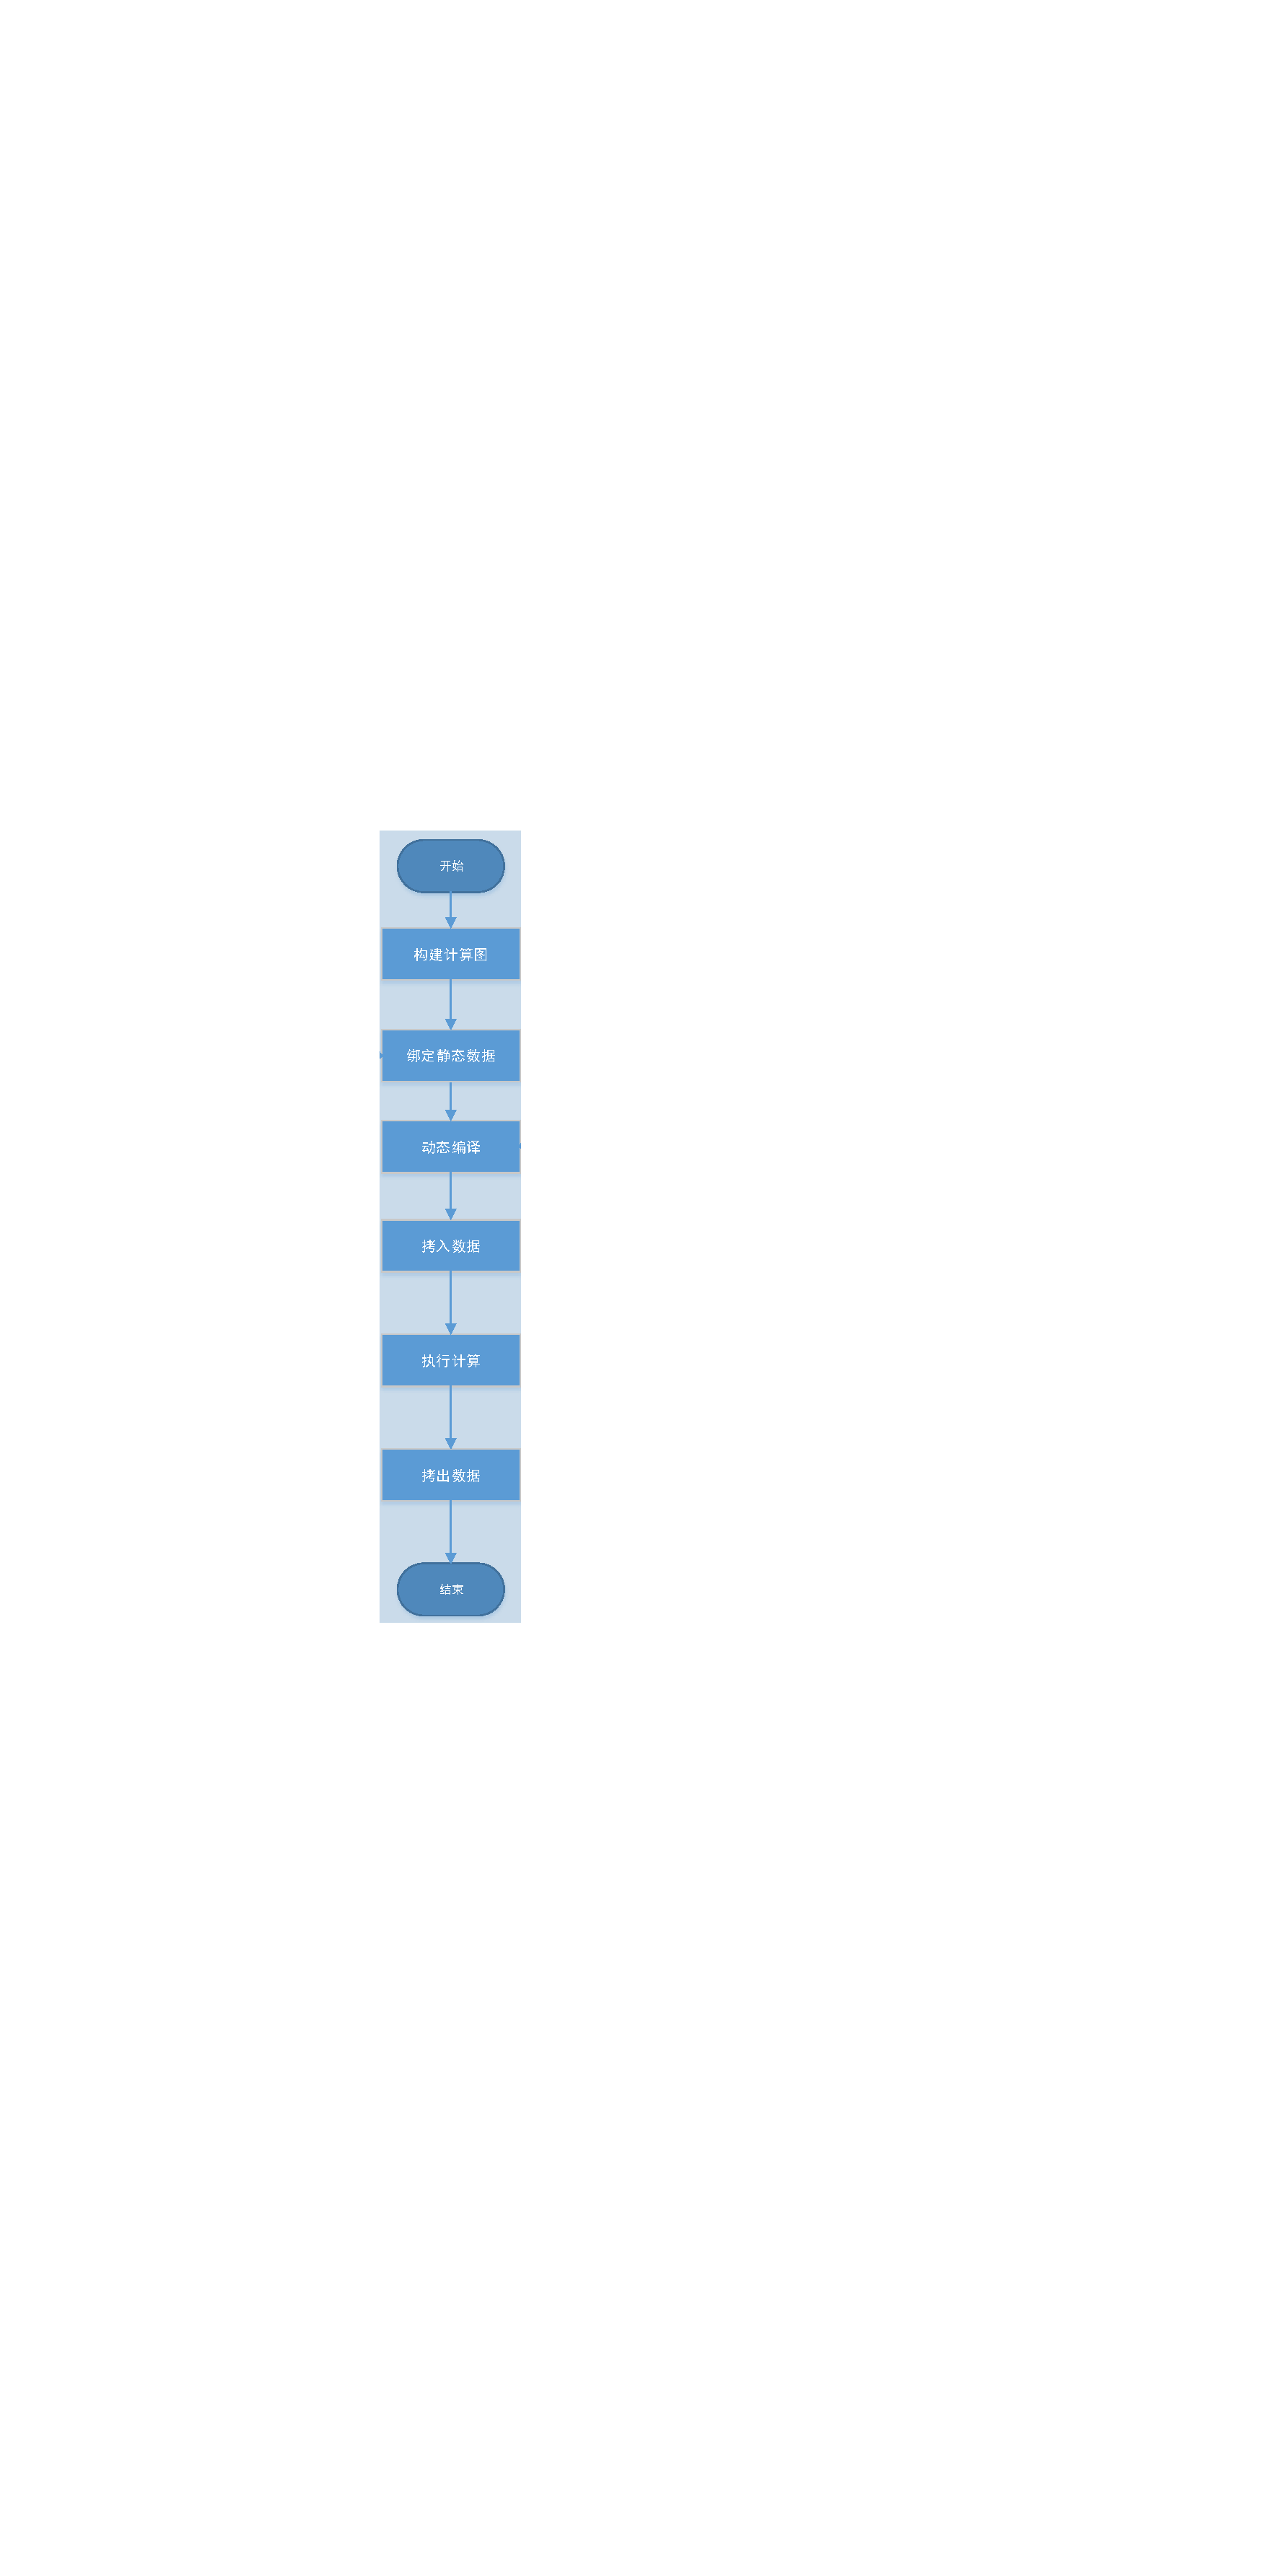
\includegraphics[width=0.18\textwidth]{figures/user_coding_process.pdf}
       \end{figure}
    \end{column}    
    \begin{column}{0.50\textwidth}
    \begin{block}{特点}
       \begin{itemize}
          \item 先声明,后编译,最后计算
          \item 动态加载输入数据
        \end{itemize}
      \end{block}
    \end{column}
  \end{columns}
\end{frame}

\begin{frame}
  \frametitle{背景技术}
  \begin{block}{3.权值量化}
    目标:通过减少表示每个权重所需的比特数来压缩静态数据的体积,而是达到压缩神经网络的目的。
  \end{block}
\end{frame}


\section{运行时流程优化设计}
\begin{frame}
  \frametitle{优化后流程}
   \begin{figure}
      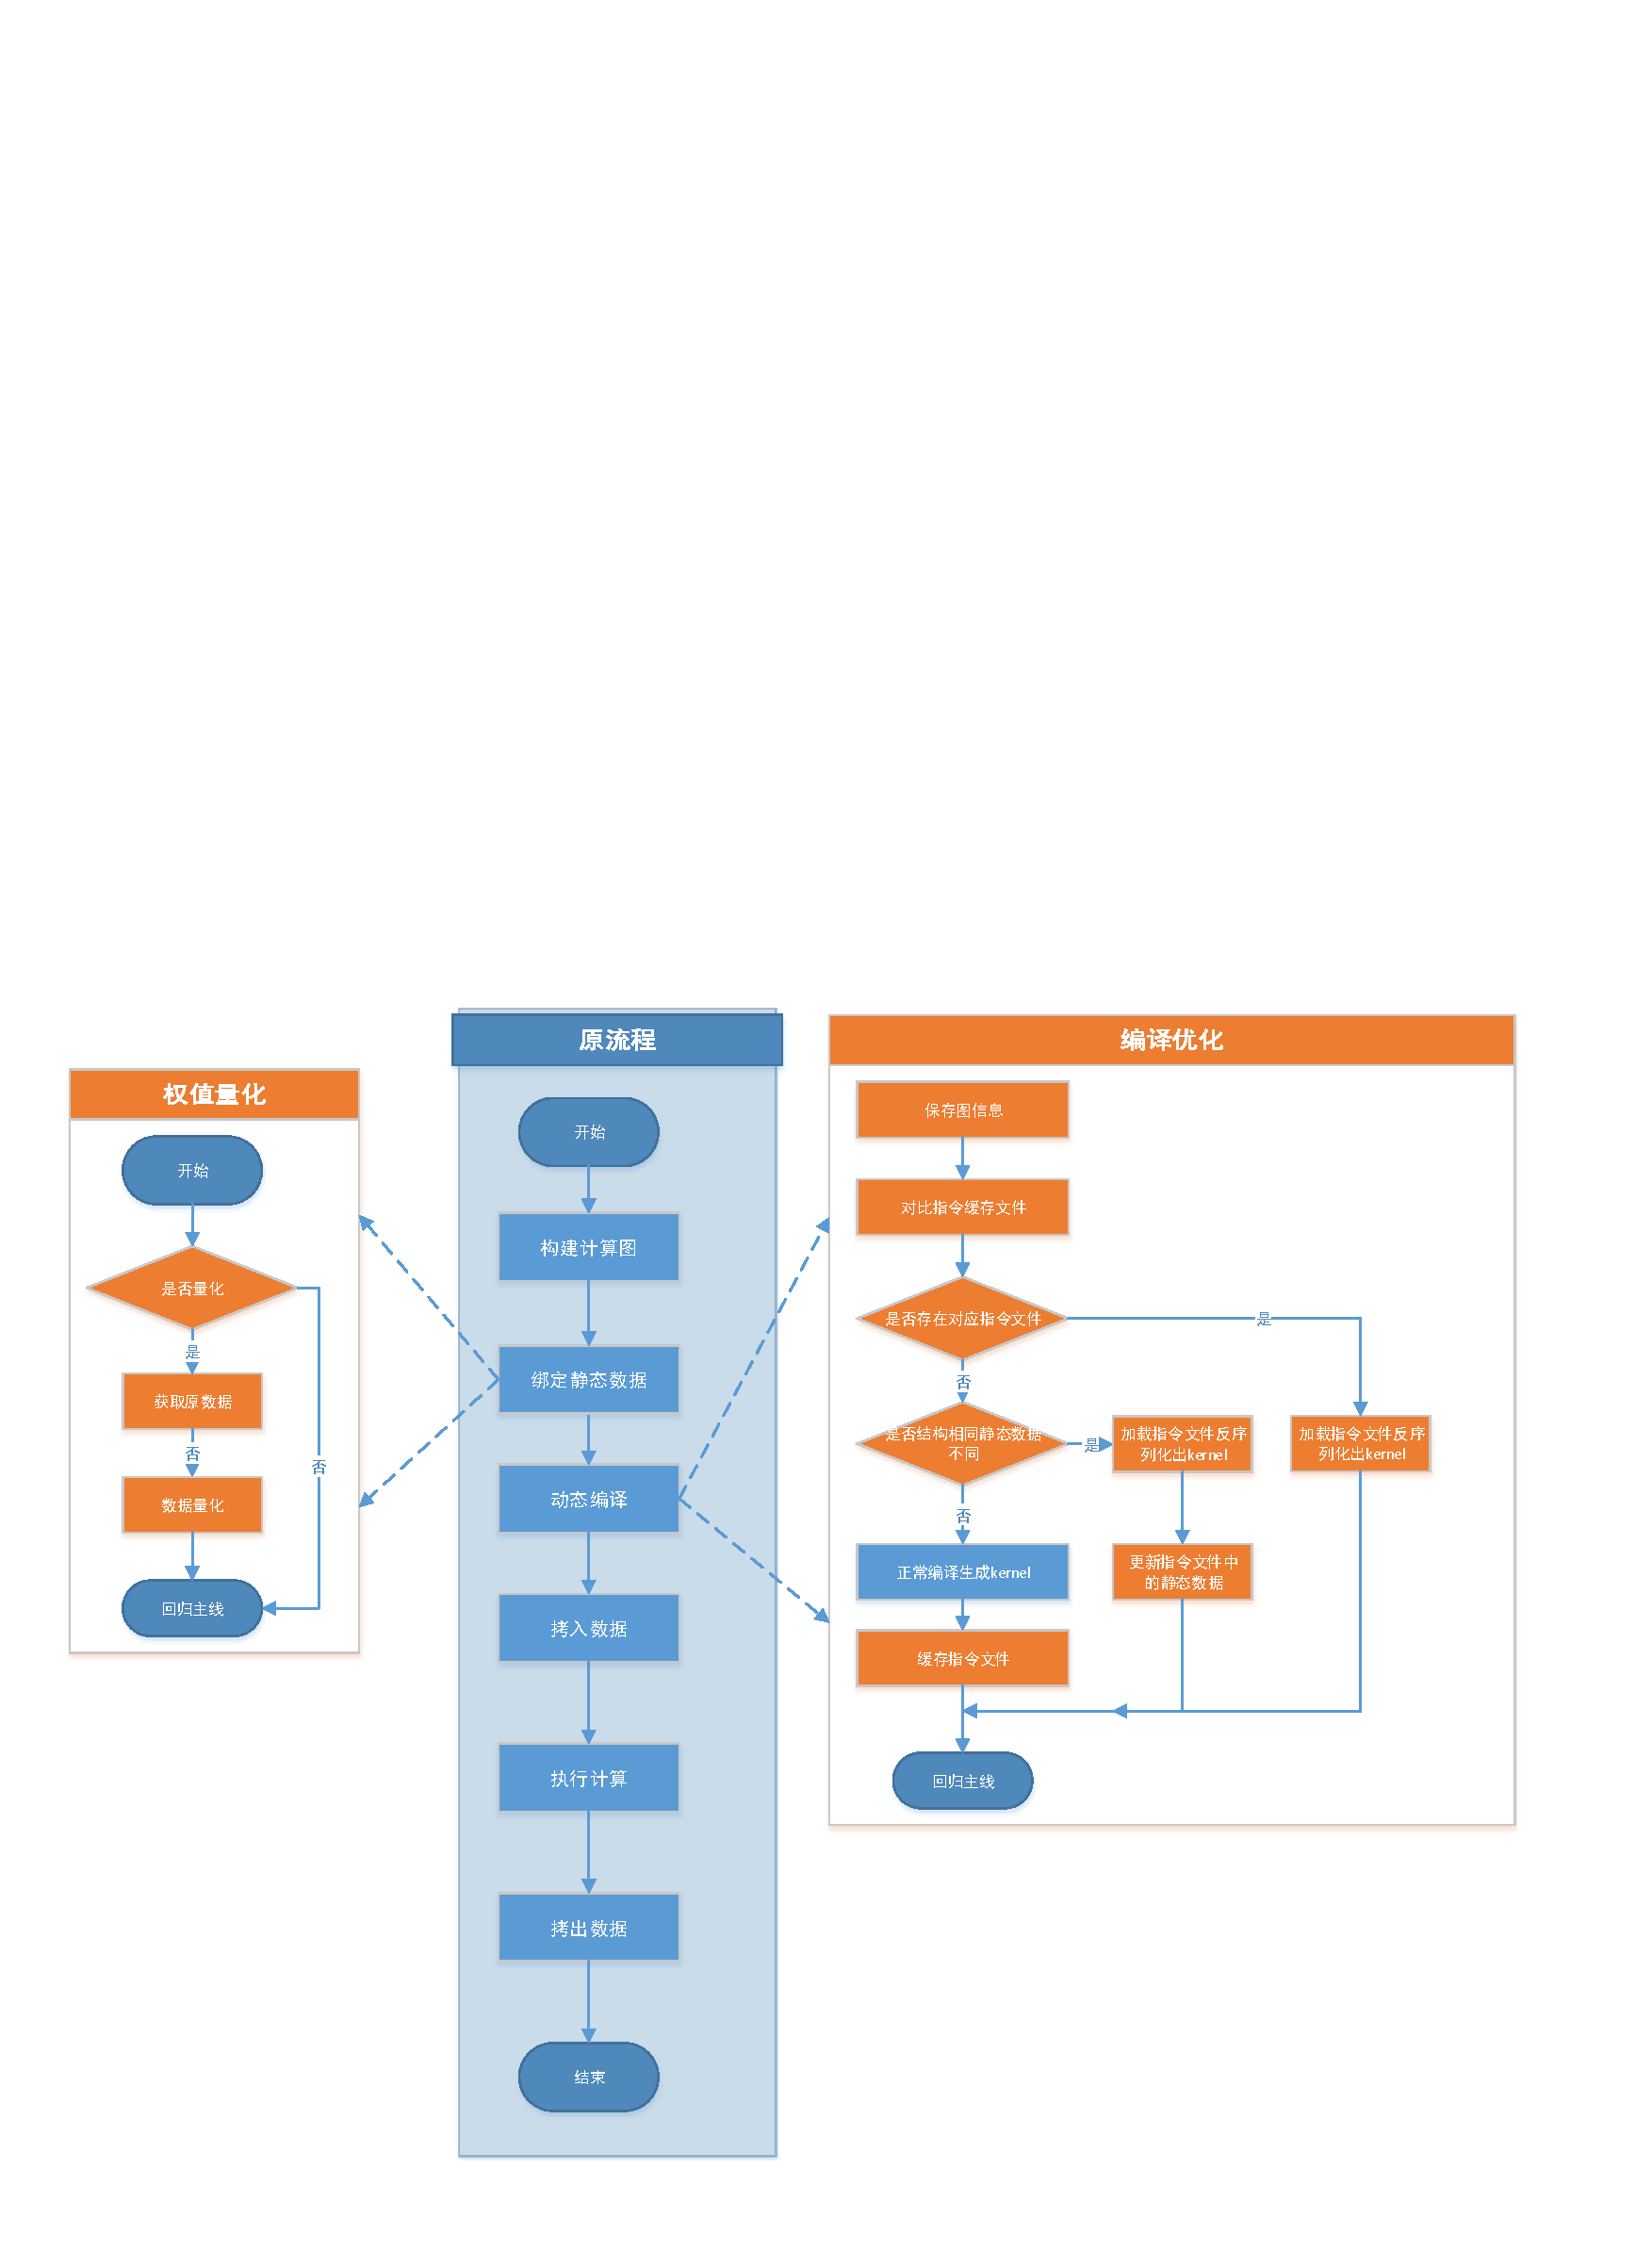
\includegraphics[width=0.75\textwidth]{figures/process_optimize.pdf}
   \end{figure}
\end{frame}


\section{功能实现}
\begin{frame}
  \frametitle{支持“离线模型”模式}
  \begin{figure}
      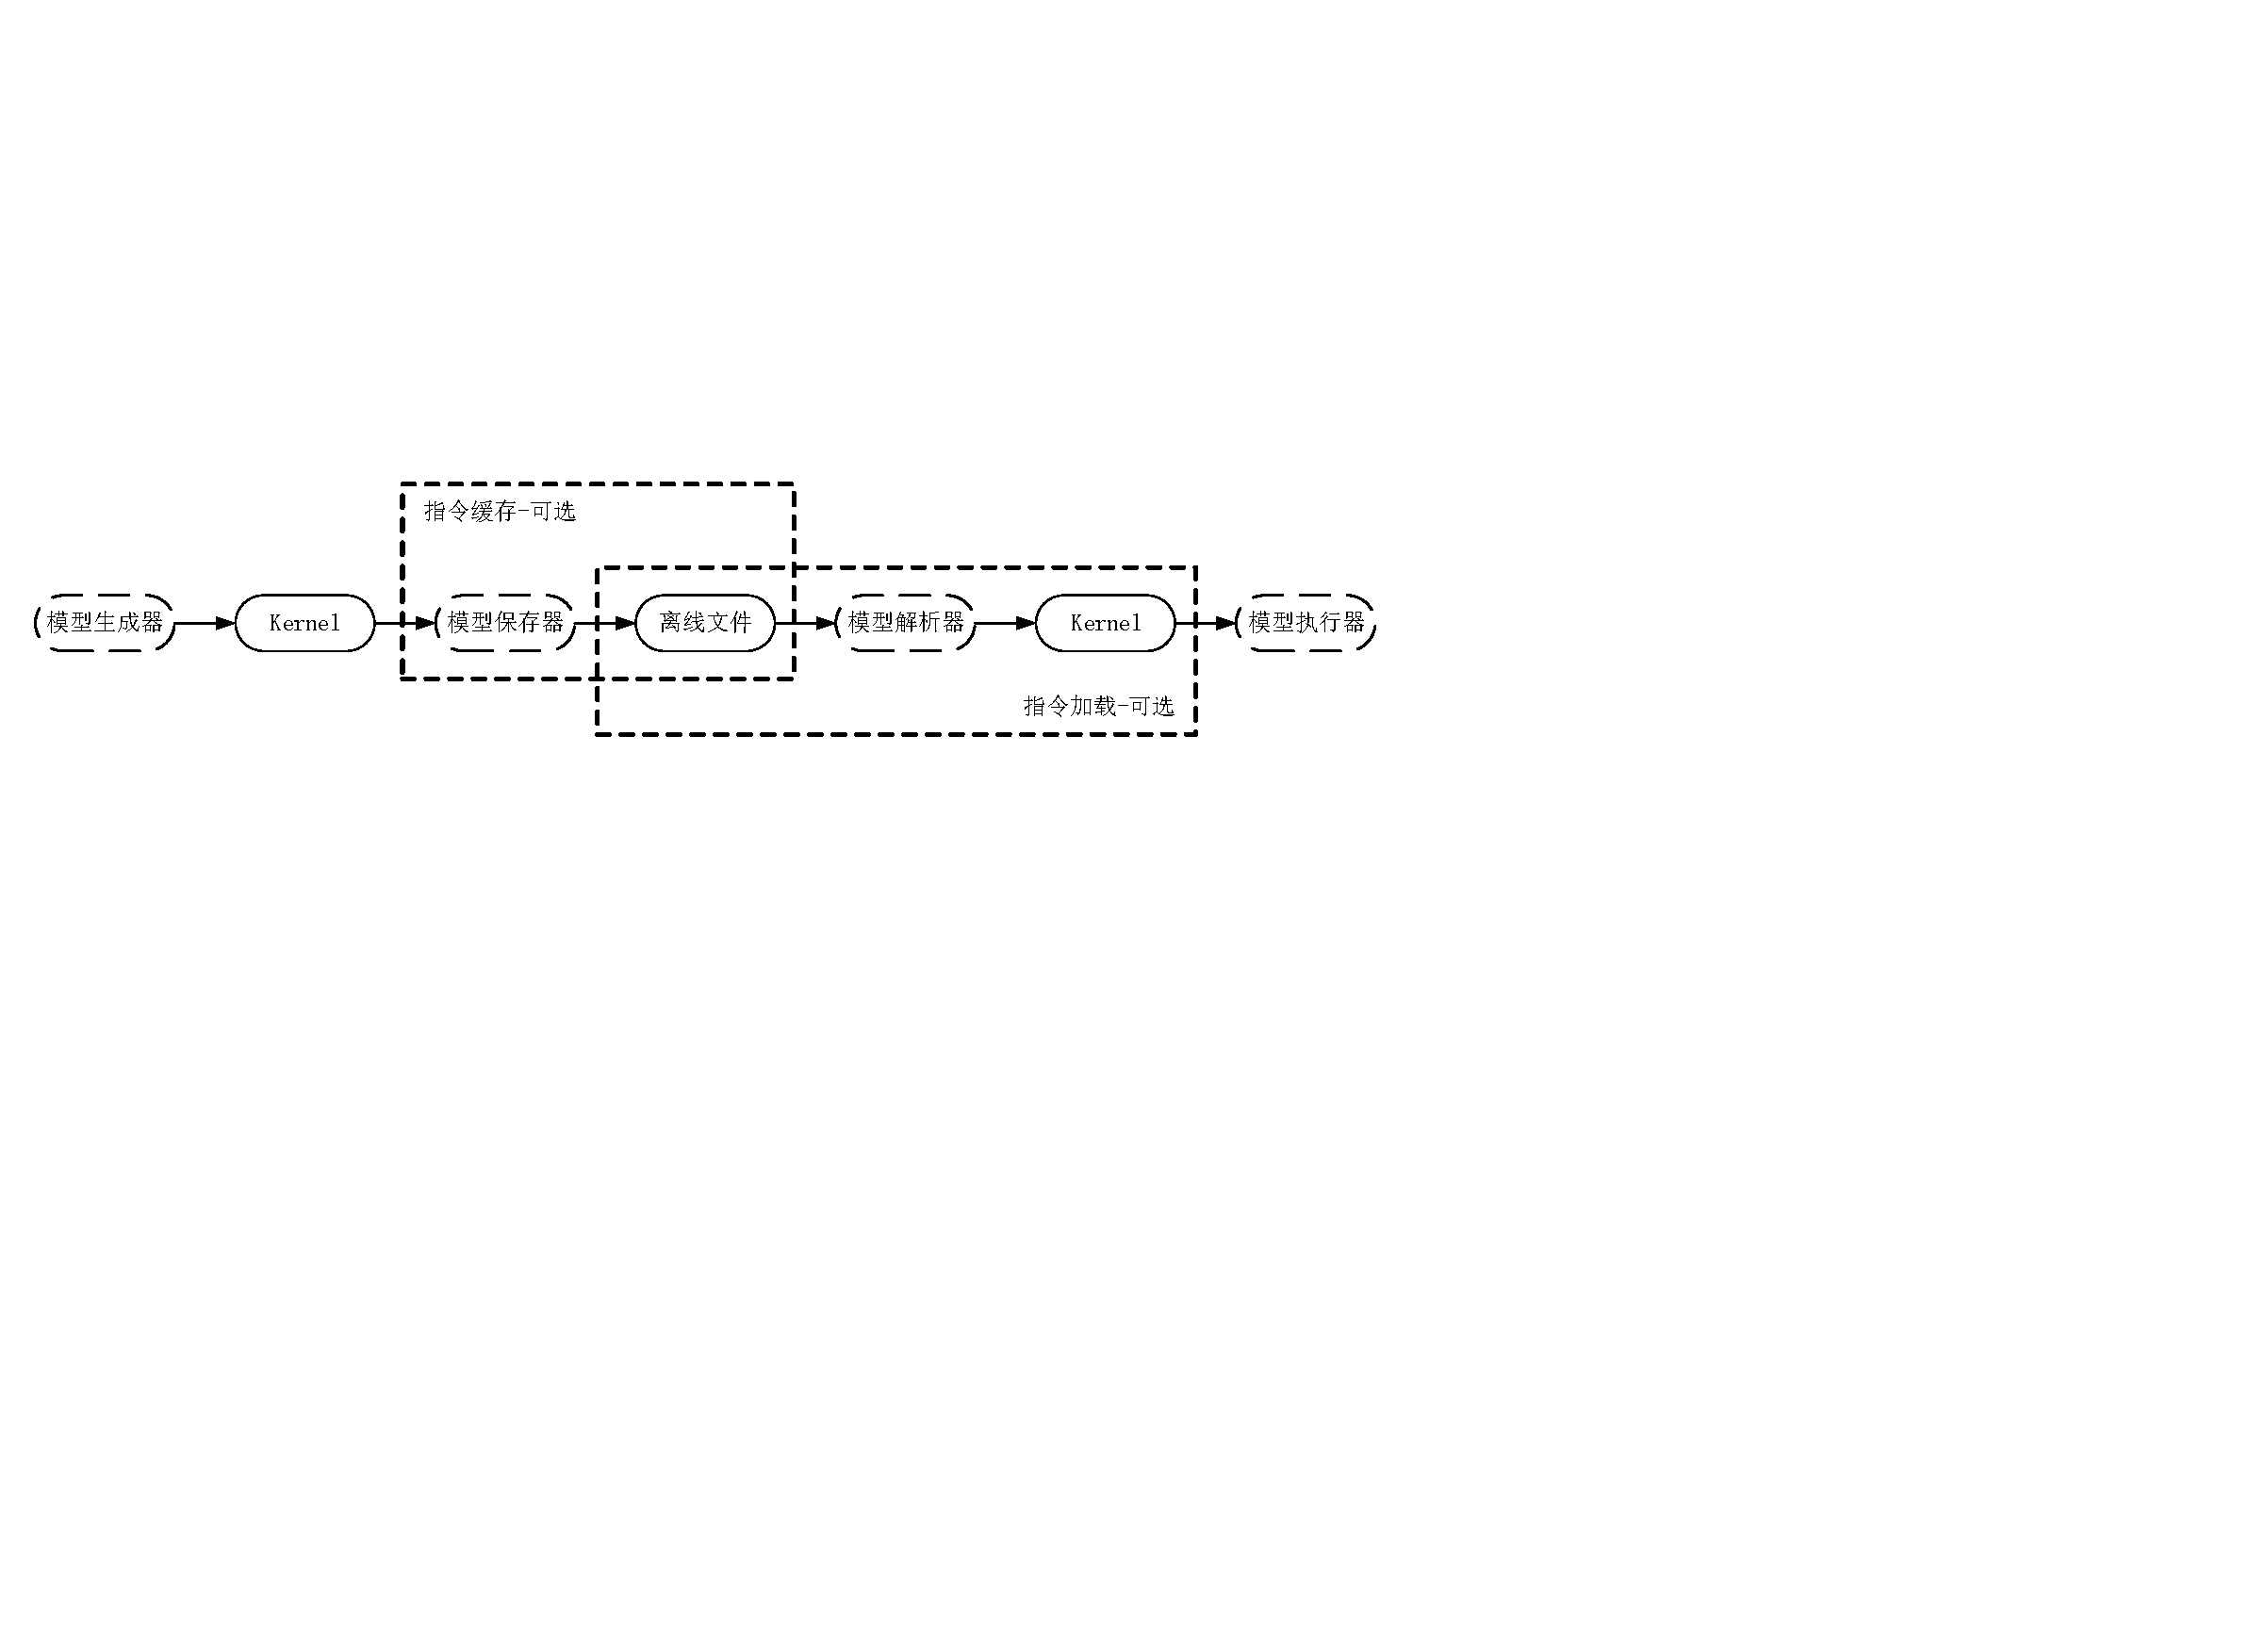
\includegraphics[width=0.6\textwidth]{figures/offline_process.pdf}
  \end{figure}
  \begin{block}{离线模型文件结构}
      \begin{figure}
         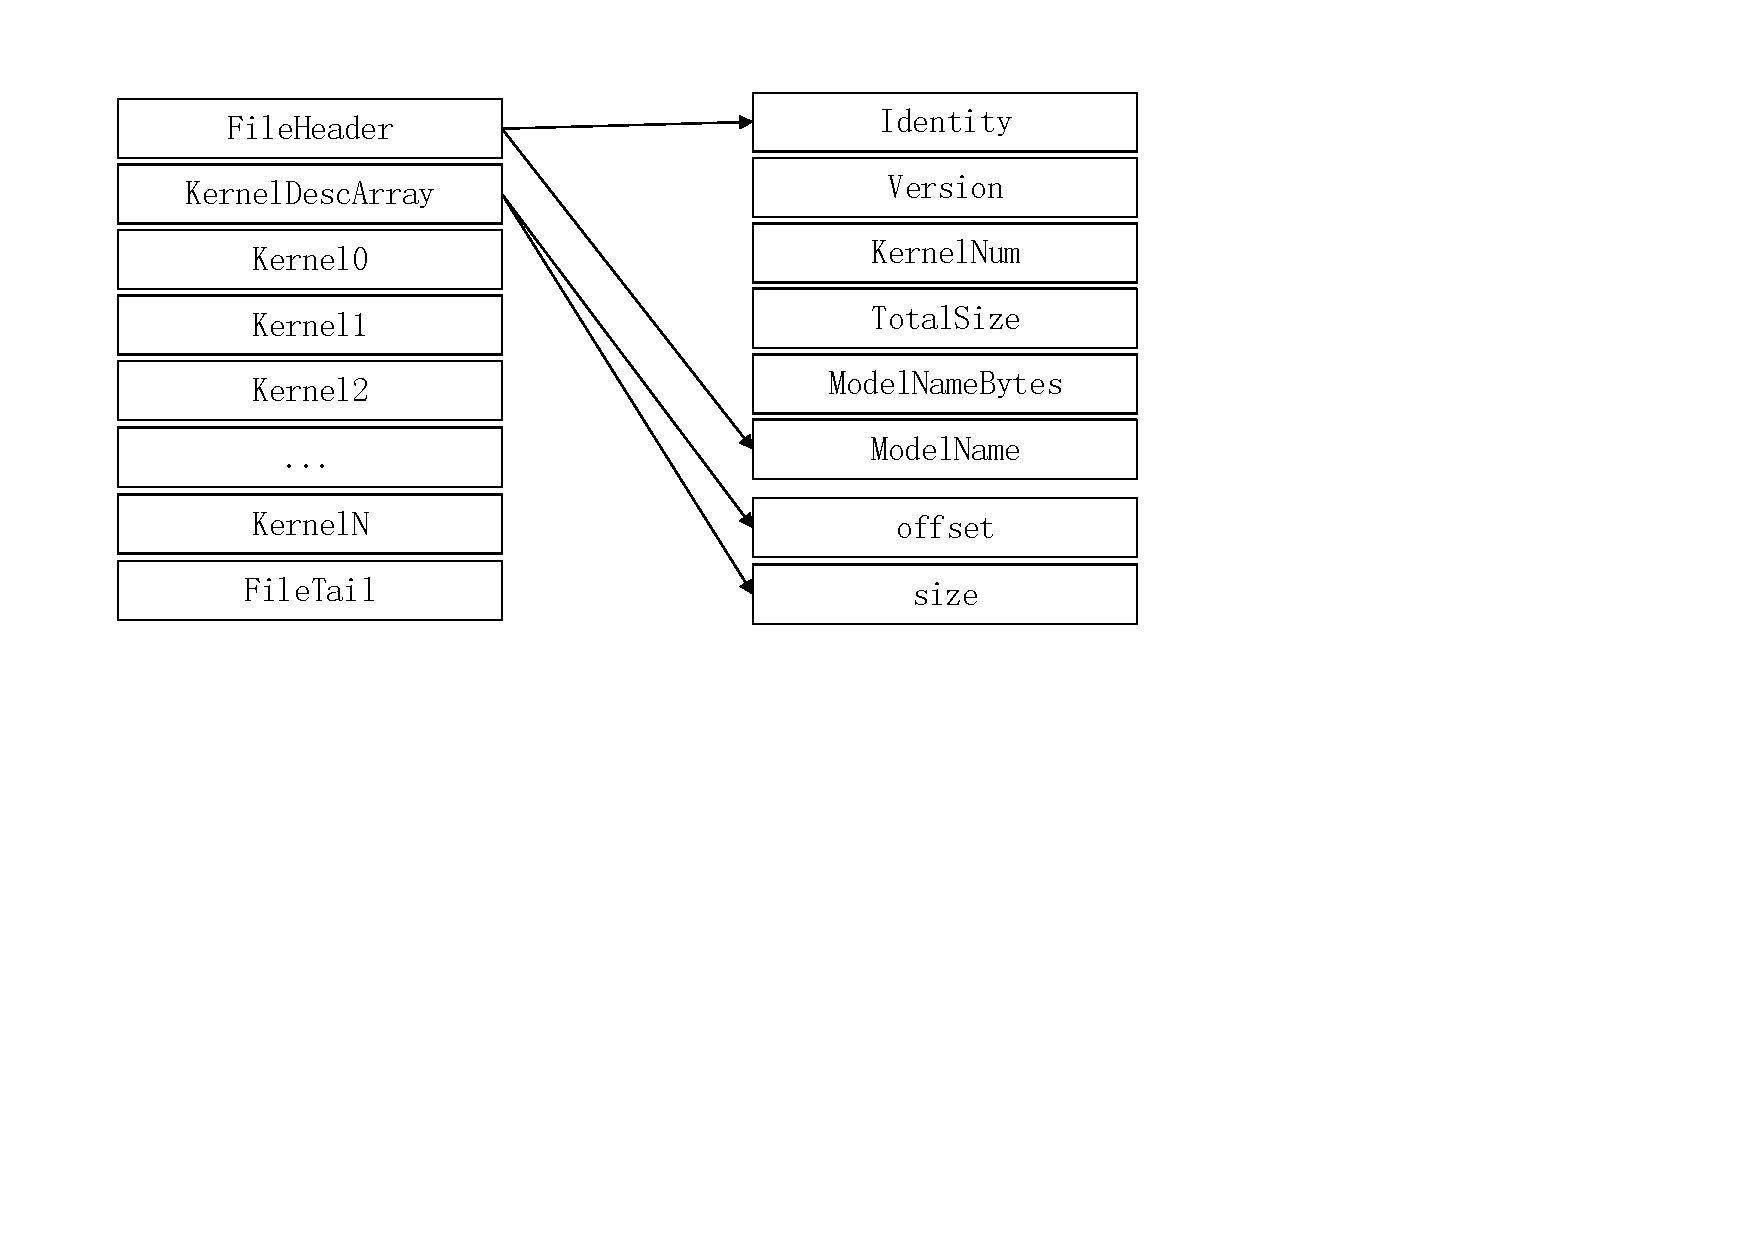
\includegraphics[width=0.75\textwidth]{figures/offmodel_struct.pdf}
      \end{figure}
  \end{block}
\end{frame}

\begin{frame}
  \frametitle{支持“离线模型”模式}
    \begin{block}{模型保存器设计}
      \begin{figure}
         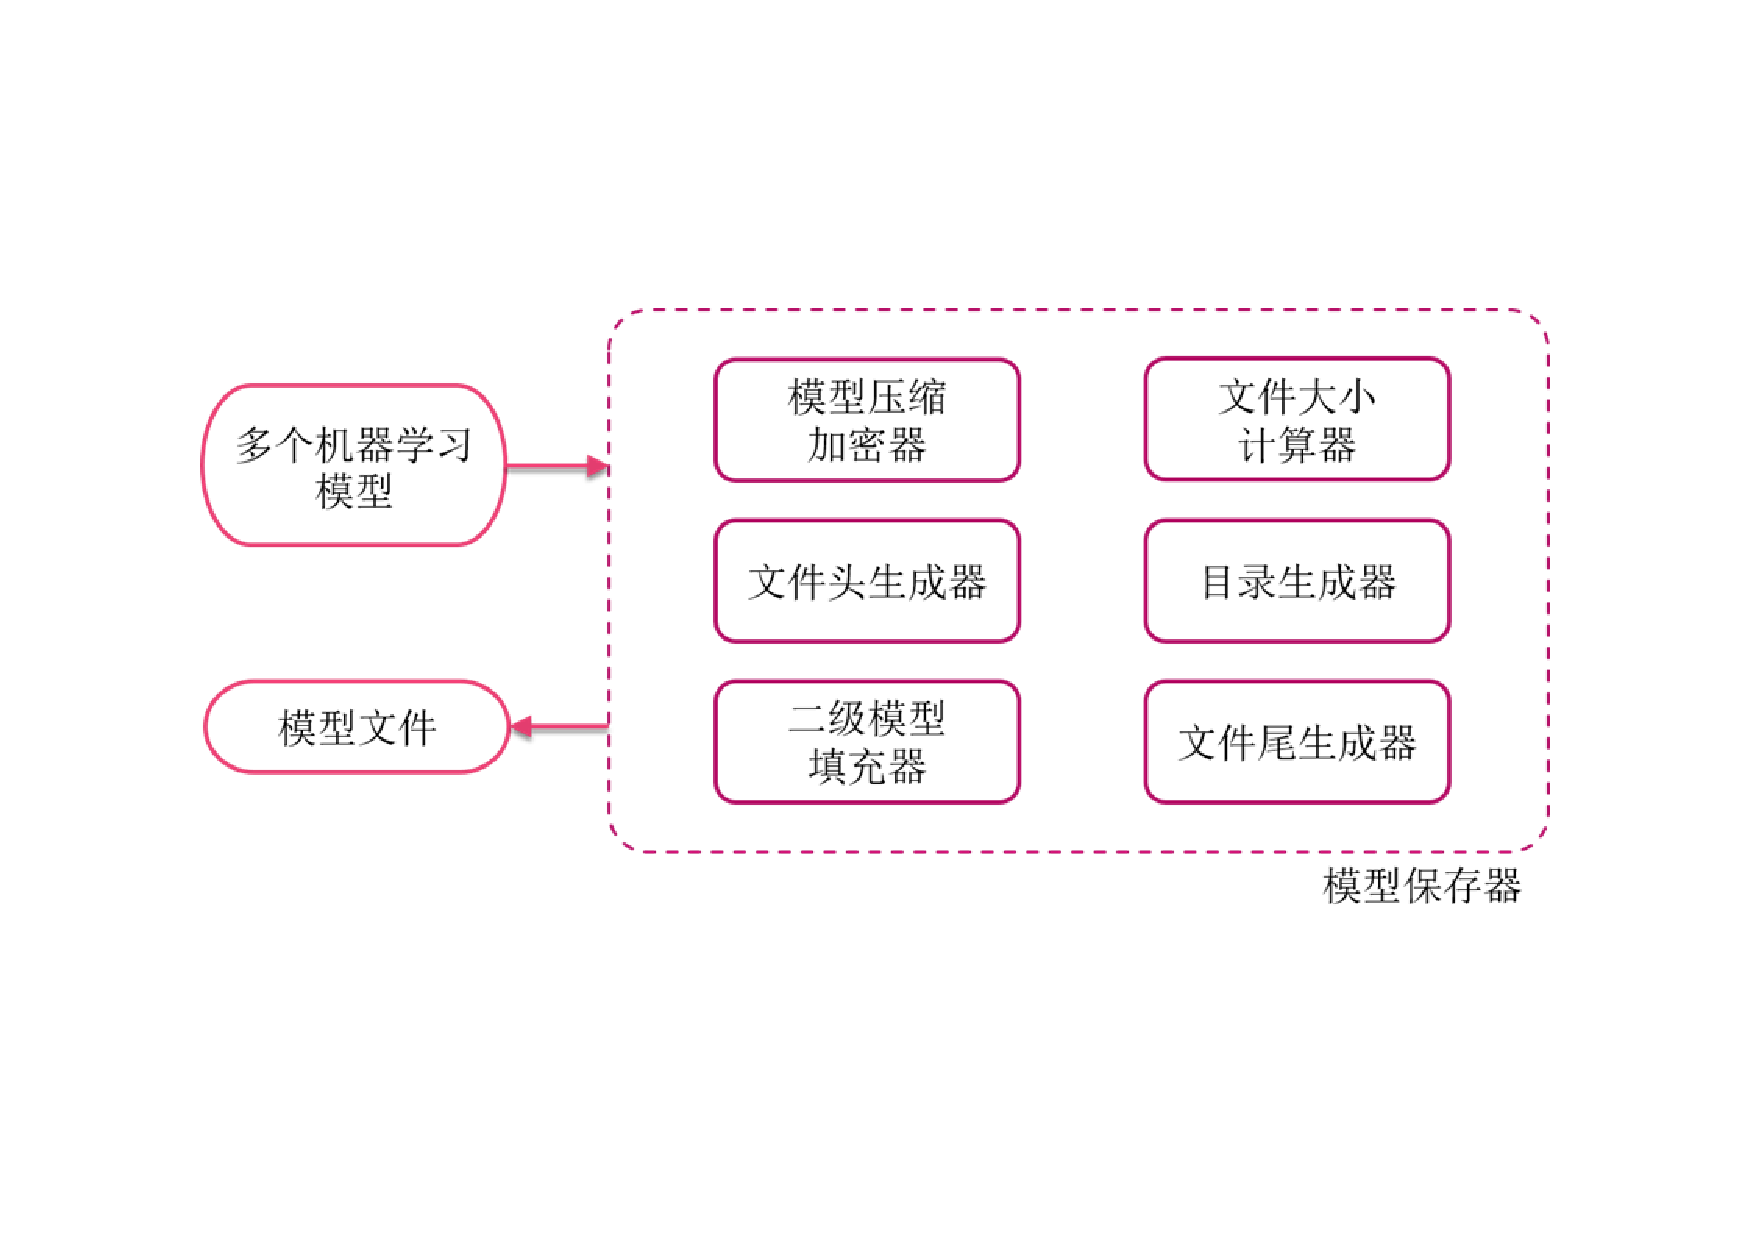
\includegraphics[width=0.75\textwidth]{figures/model_save.pdf}
      \end{figure}  
    \end{block}
\end{frame}

\begin{frame}
  \frametitle{支持“离线模型”模式}
    \begin{block}{模型解析器设计}
      \begin{figure}
         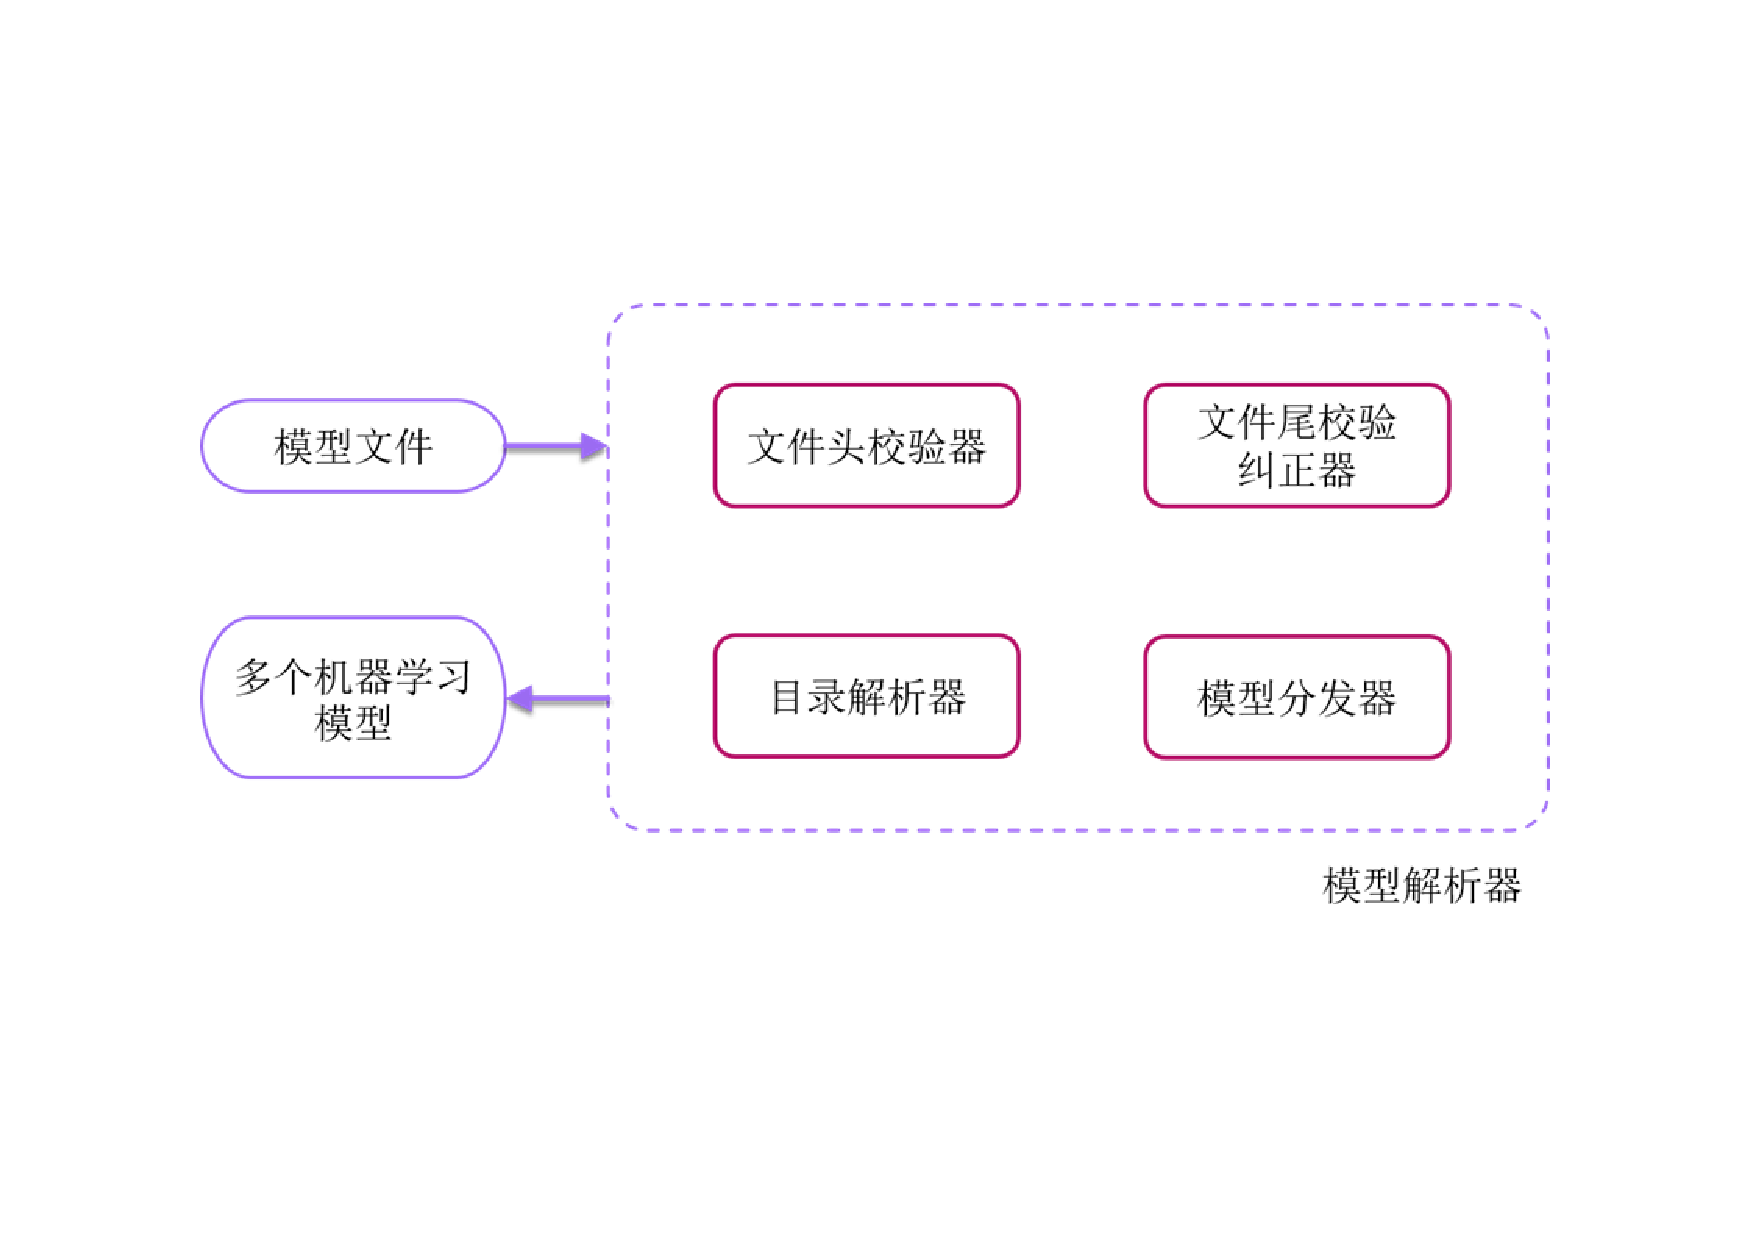
\includegraphics[width=0.75\textwidth]{figures/model_praser.pdf}
      \end{figure}  
    \end{block}
\end{frame}

\begin{frame}
  \frametitle{避免重复编译}
    \begin{block}{核心功能}
        \begin{itemize}
          \item 保存计算图信息,包括编译环境信息,网络结构信,静态数据信息
          \item 权值替换
          \item 指令替换
        \end{itemize}
    \end{block}
\end{frame}

\begin{frame}
  \frametitle{避免重复编译}
     \begin{block}{json文件展示图}
         \begin{columns}
             \begin{column}{0.3\textwidth}
                \begin{figure}
		        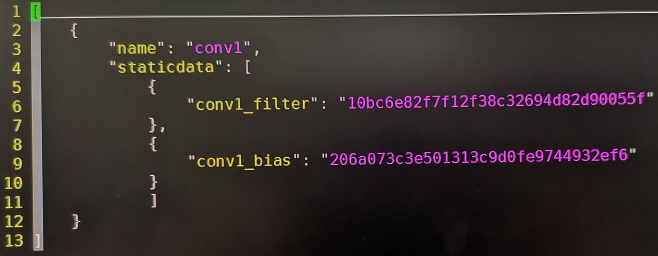
\includegraphics[width=0.9\textwidth]{figures/static_info.png}
                \end{figure}
             \end{column}    
            \begin{column}{0.3\textwidth}
                \begin{figure}
		        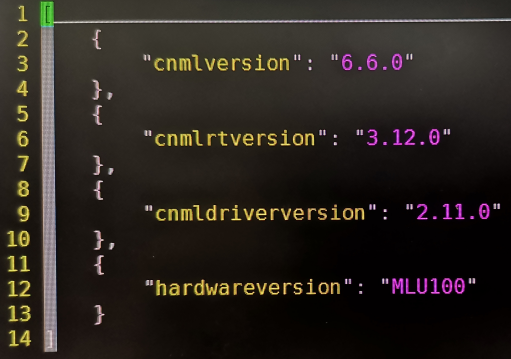
\includegraphics[width=0.9\textwidth]{figures/env_info.png}
                \end{figure}
            \end{column}
            \begin{column}{0.4\textwidth}
                \begin{figure}
		        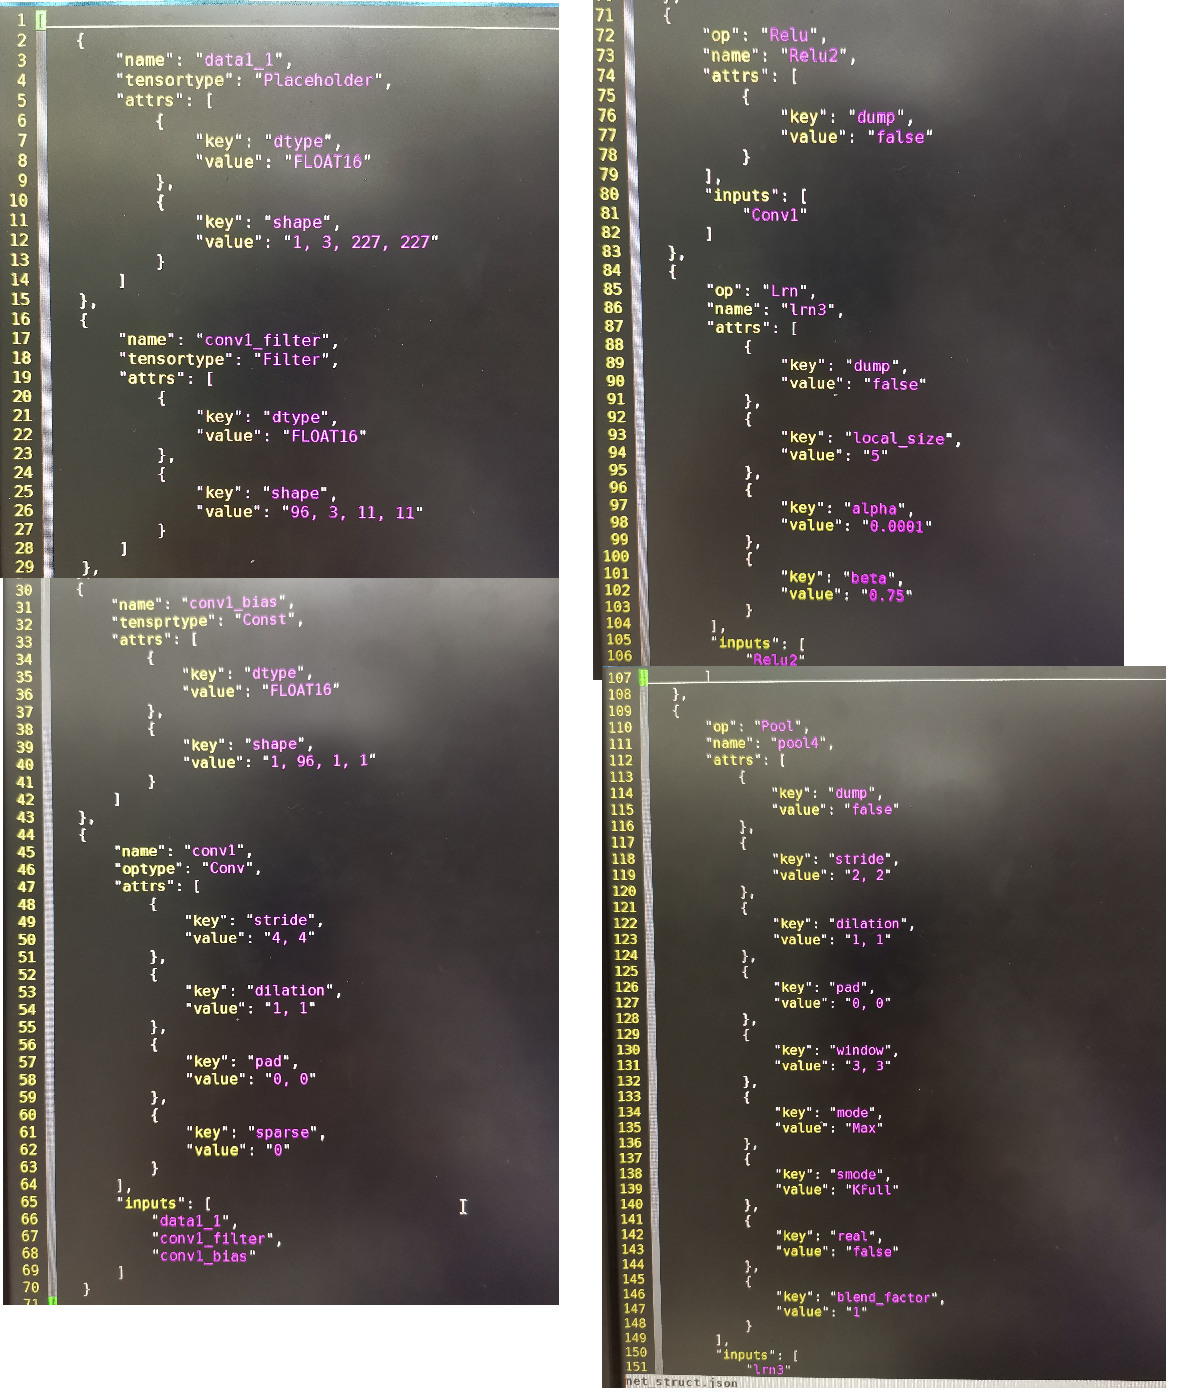
\includegraphics[width=1.0\textwidth]{figures/net_struct.png}
                \end{figure}
            \end{column}
     \end{columns}
  \end{block}
\end{frame}

\begin{frame}
  \frametitle{避免重复编译}
    匹配离线模型流程
    \begin{figure}
	  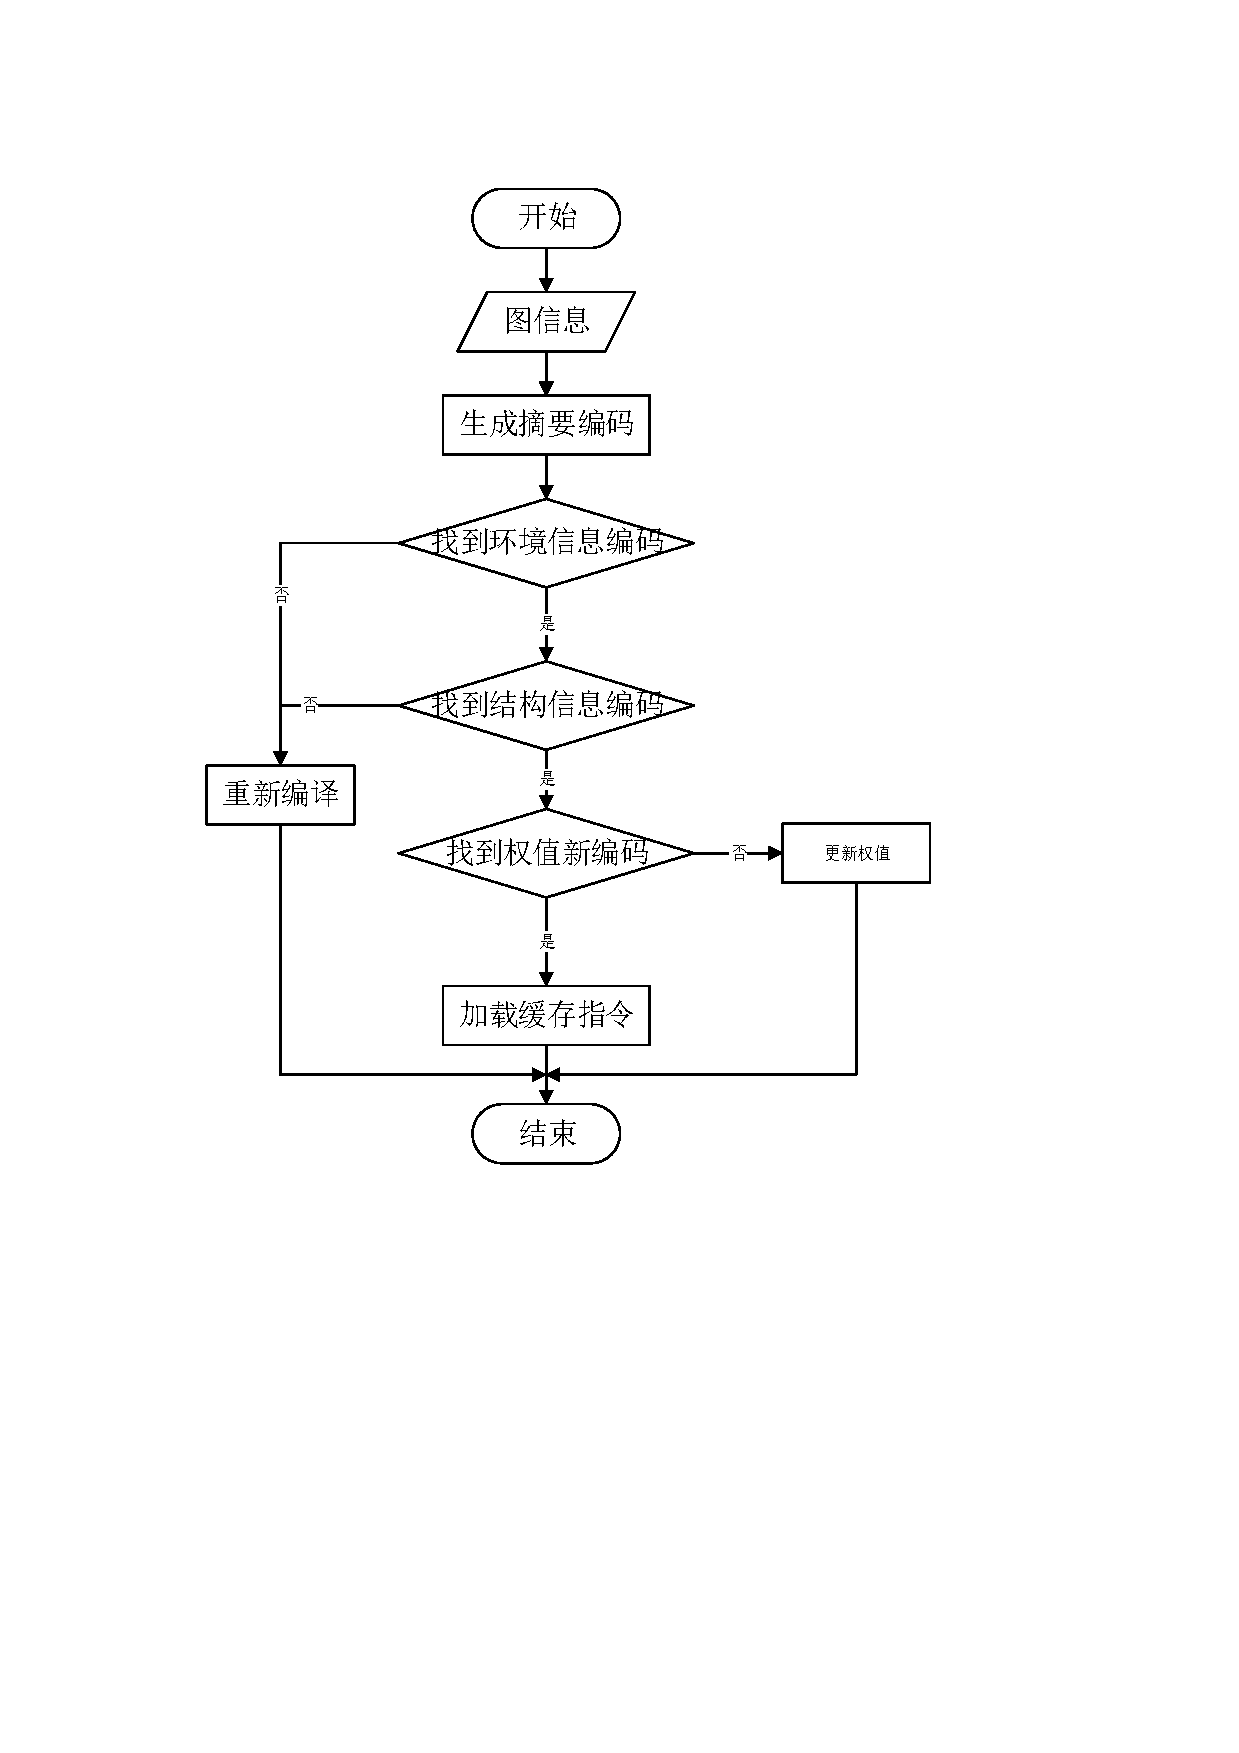
\includegraphics[width=0.4\textwidth]{figures/get_cache_model.pdf}
    \end{figure}
\end{frame}

\begin{frame}
  \frametitle{避免重复编译}
    权值替换过程
    \begin{figure}
	  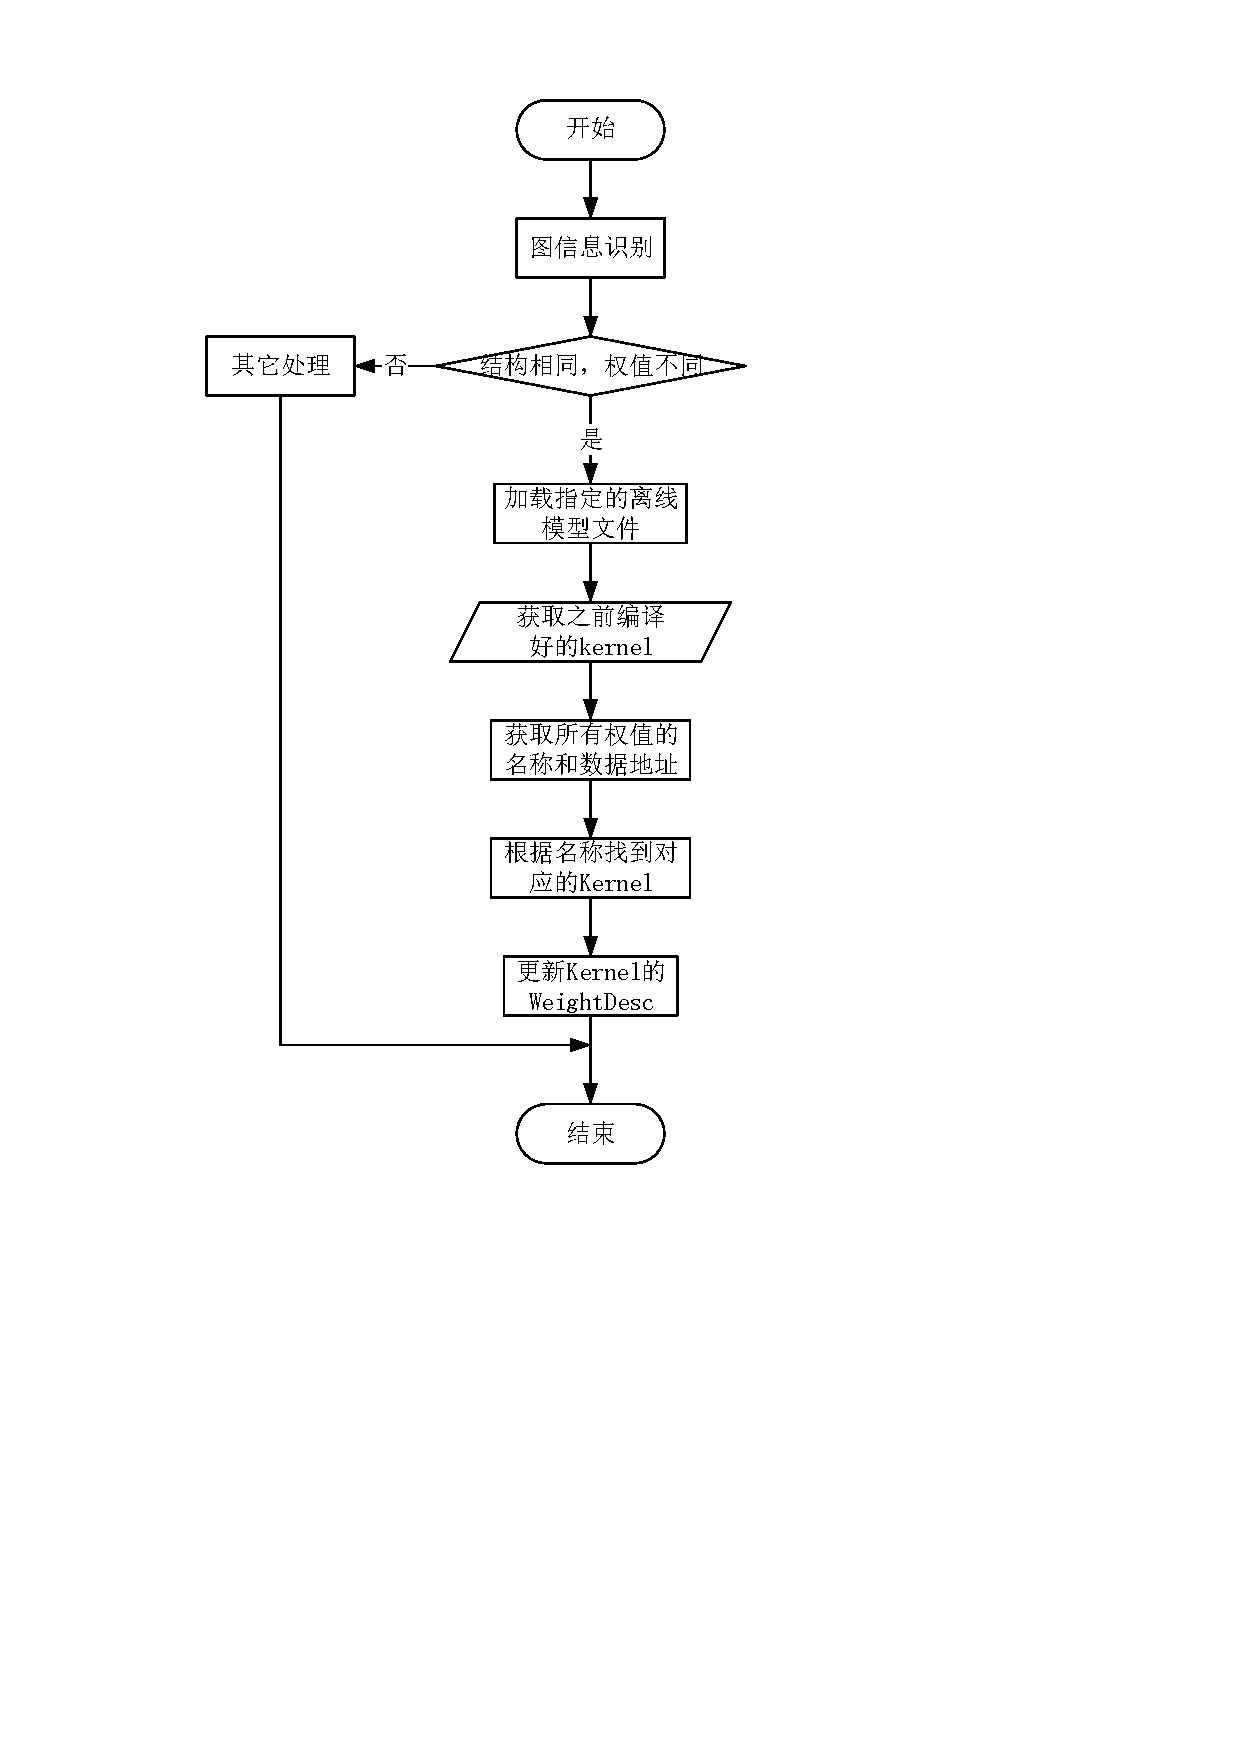
\includegraphics[width=0.28\textwidth]{figures/weight_replace_process.pdf}
    \end{figure}
\end{frame}

\begin{frame}
  \frametitle{权值量化}
    权值替换过程
    \begin{figure}
	  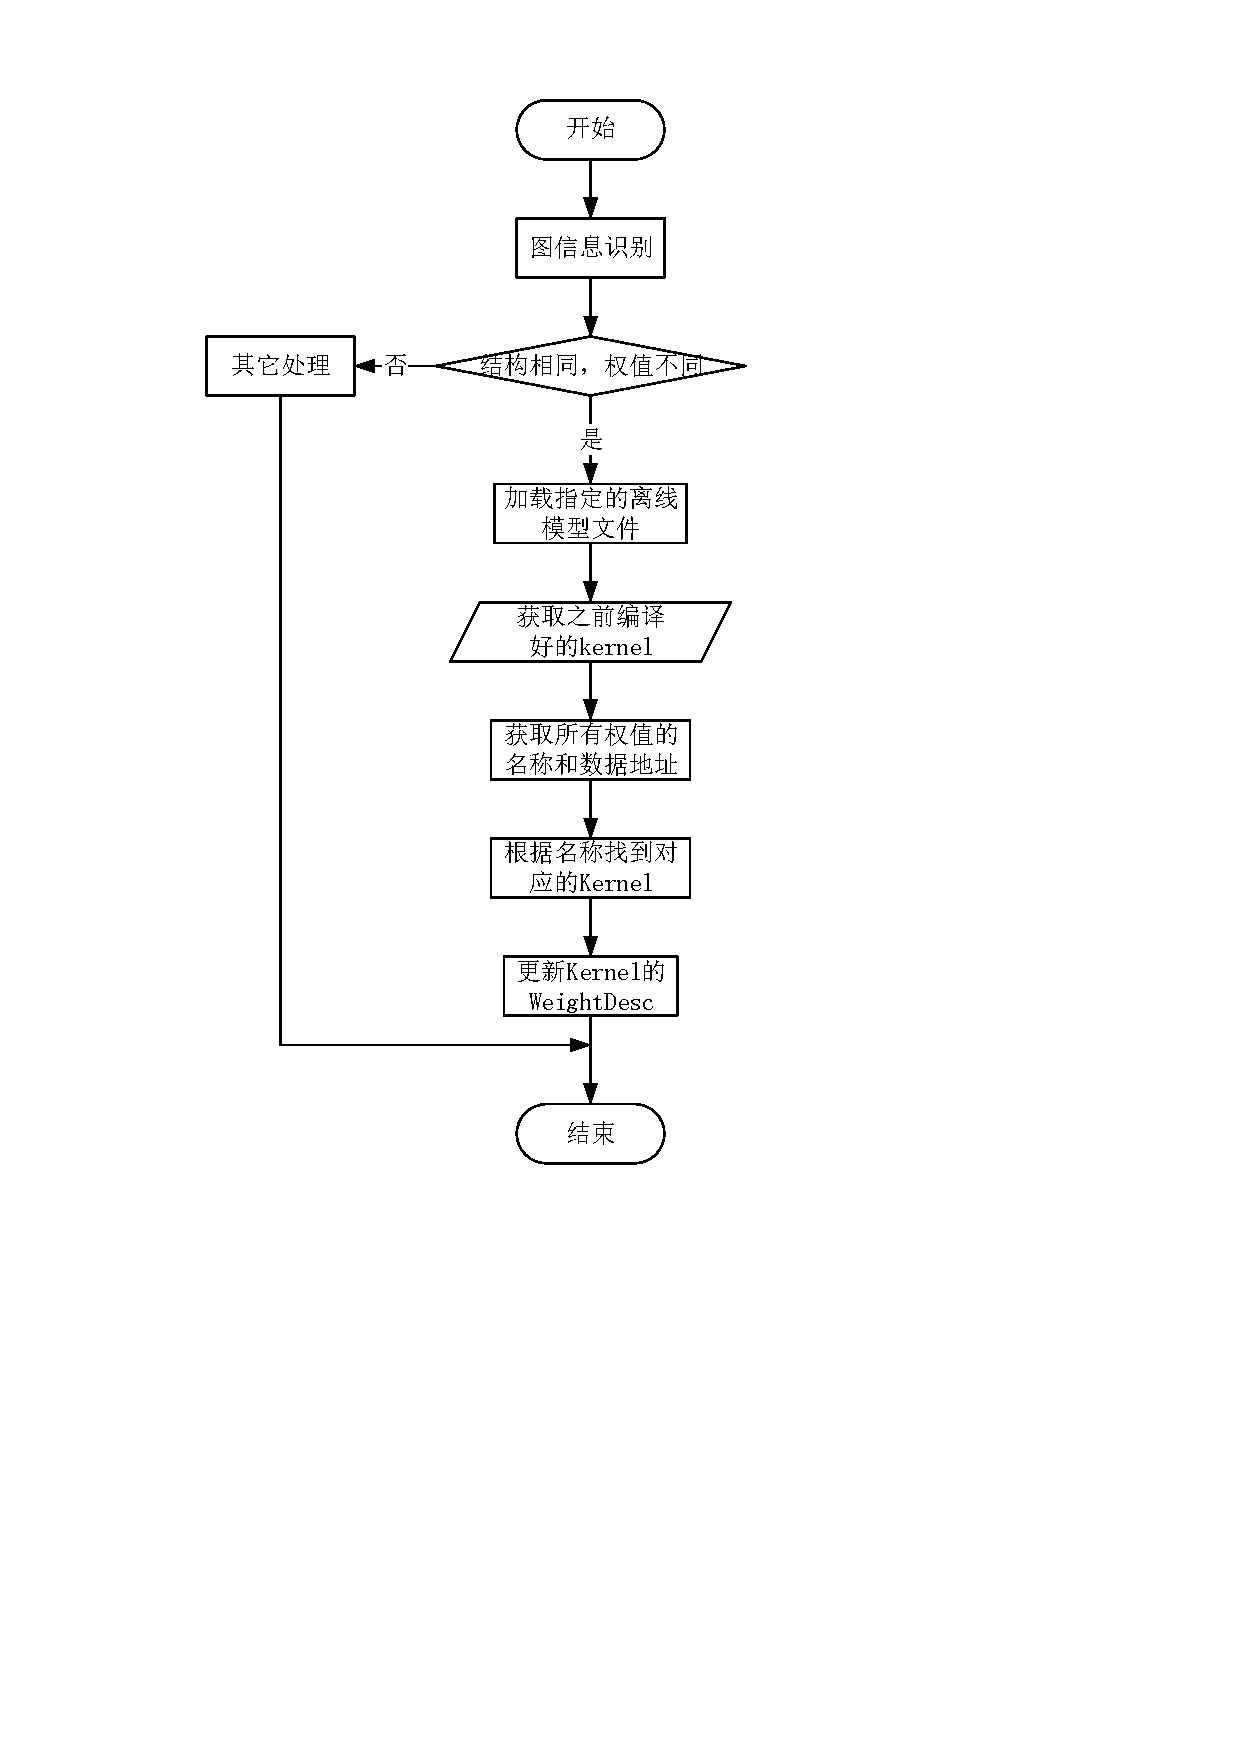
\includegraphics[width=0.28\textwidth]{figures/weight_replace_process.pdf}
    \end{figure}
\end{frame}

\begin{frame}
  \frametitle{权值量化}
    权值量化过程
    \begin{figure}
	  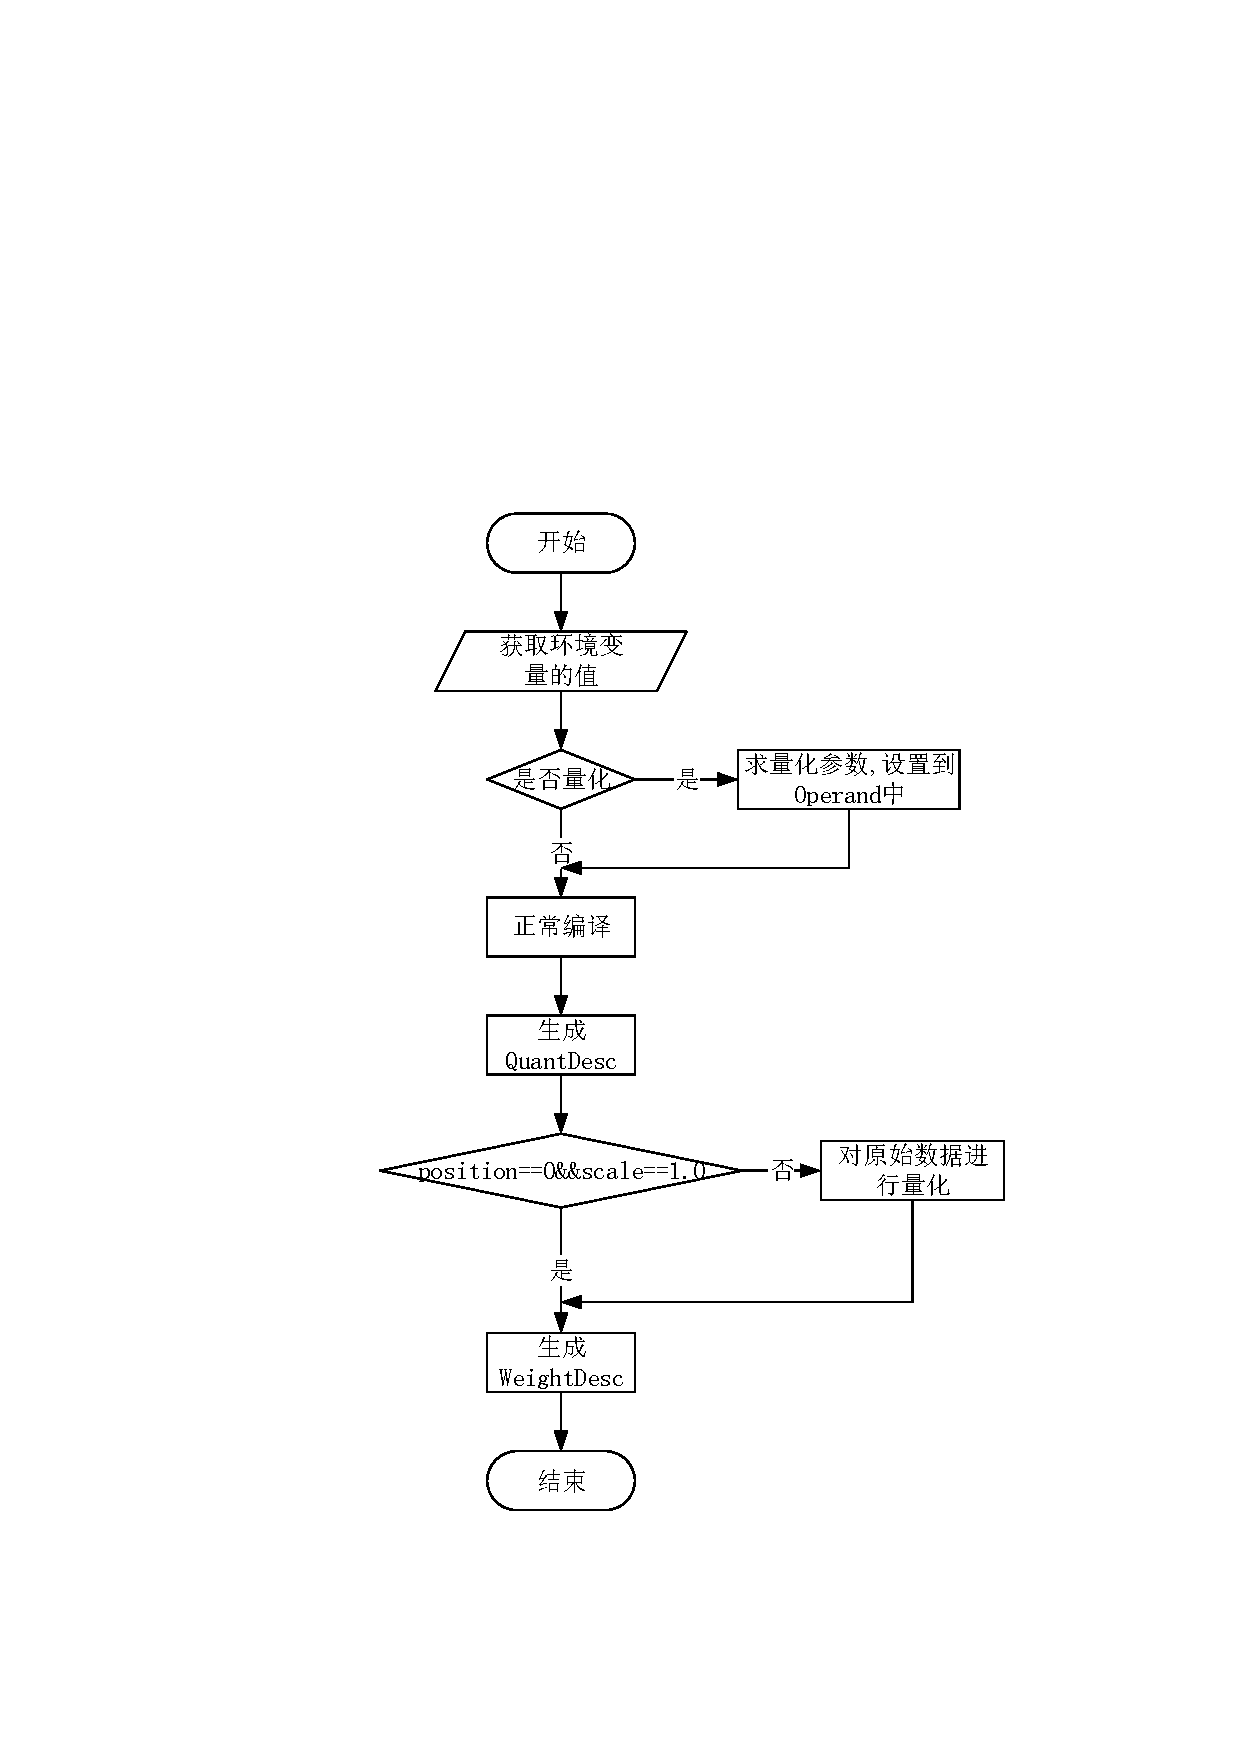
\includegraphics[width=0.28\textwidth]{figures/weight_quant_process.pdf}
    \end{figure}
\end{frame}

\section{测试结果}

\begin{frame}
  \frametitle{测试环境}
    \begin{figure}
	 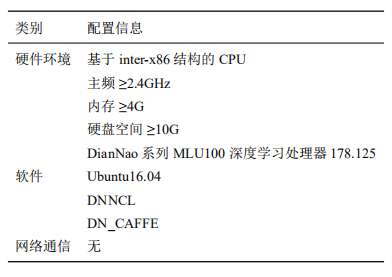
\includegraphics[width=0.7\textwidth]{figures/test_env.png}
    \end{figure}
\end{frame}

\begin{frame}
  \frametitle{指令缓存测试结果}
    \begin{figure}
	 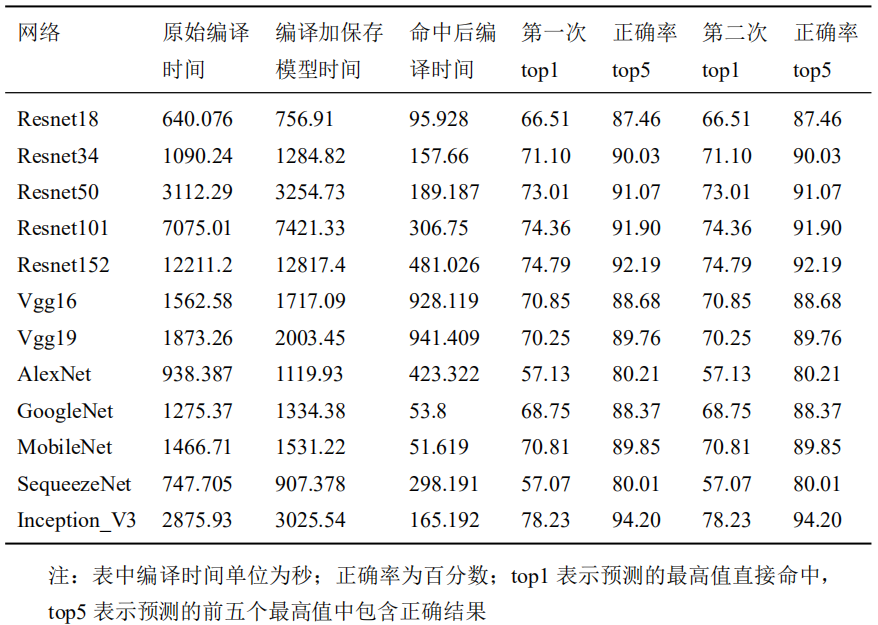
\includegraphics[width=0.7\textwidth]{figures/inst_cache.png}
    \end{figure}
\end{frame}


\begin{frame}
  \frametitle{权值量化测试结果}
    \begin{figure}
	 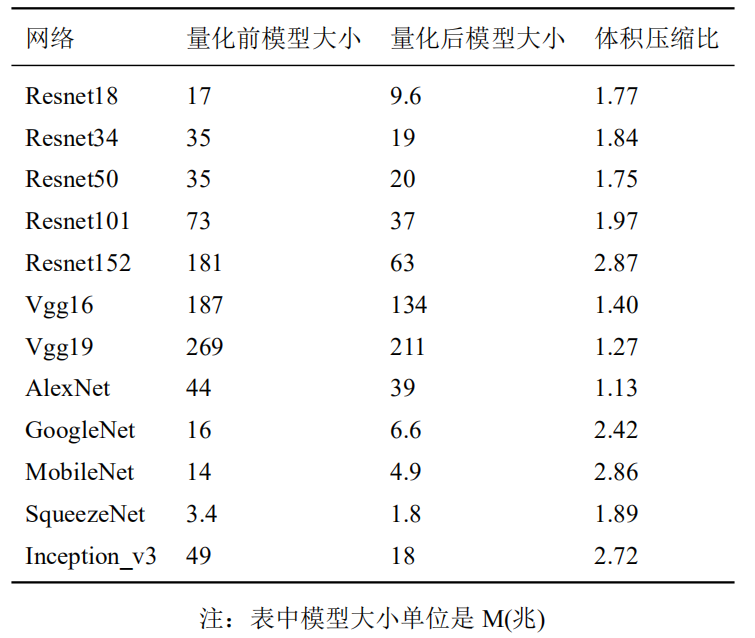
\includegraphics[width=0.7\textwidth]{figures/quant_bulk.png}
	 % \caption{带追踪模块的多通道目标检测效果图}
    \end{figure}
\end{frame}


\begin{frame}
  \frametitle{权值量化测试结果}
    \begin{figure}
	 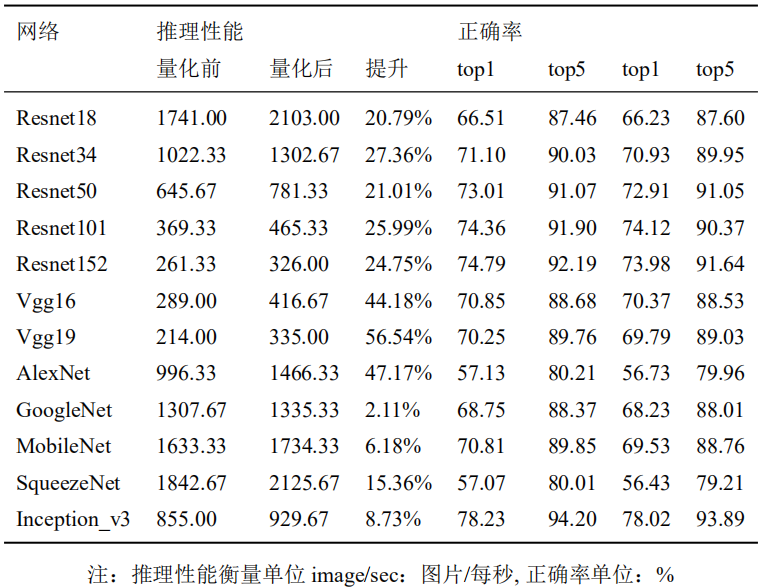
\includegraphics[width=0.7\textwidth]{figures/quant_result.png}
	 % \caption{带追踪模块的多通道目标检测效果图}
    \end{figure}
\end{frame}


\section{总结与展望}
\begin{frame}
  \frametitle{总结与展望}
    \begin{block}{总结}
	 \begin{itemize}
          \item 实现了一种面向神经网络模型的指令存储和加载技术,能将深度学习框架计算任务对应的指令信息和数据信息离线保存到本地文件中,然后在运行时支持从文    件中加载之前编译好的指令结合当前的输入数据进行计算。
          \item 实现了一种神经网络存储与识别技术,结合权值更新技术,能极大的提高缓存的命中率,避免相同网络的重复编译
          \item 实现了一种神经网络模型的压缩技术,对权值数据做量化处理,在保持精度损失在可接受的范围内能大幅减少神经网络模型的存储空间和部署时所占用的内存资源
     	\end{itemize}
   \end{block}
\end{frame}

\begin{frame}
  \frametitle{总结与展望}
    \begin{block}{展望}
      \begin{block}{还可以进一步进行网络压缩}
	   \begin{itemize}
          \item 网络剪枝
          \item 对量化后的权重进行霍夫曼编码
          \item 低秩因子分解
     	   \end{itemize}
     \end{block}
     \begin{block}{基于“离线模型”模式}
	   \begin{itemize}
          \item 可以支持维度可变
     	   \end{itemize}
     \end{block}
   \end{block}
\end{frame}  

\begin{frame}
  \centerline{\Large Thanks! Q\&A.}
\end{frame}


\end{document}
